\chapter{State of the Art}
\label{chapter:state_of_the_art}

This chapter aims to provide a description and overview of important concepts and protocols of \acf{bas}, \acf{iot} as well as event processing. For each topic there will be a review of the different technologies, how they interact and how they differ from each other.

All of the topics addressed in this chapter contributed to the solution presented, either in a combination of different technologies or choosing from similar ones.

\section{\acf{bas}}

A \acf{bas} consists in the automatic control and monitoring of building services such as lighting, heating, ventilation, air conditioning, and more. The main purpose of \ac{bas} is to improve the comfort of the building's occupants, while decreasing significantly the operational costs and energy consumption. This is achieved using the information gathered by a wide set of sensors, that is used to control building equipment behaviour such as lighting, \ac{hvac}, shutters, and others \cite{Brambley2005}. This information can also be used to prevent and react quickly to emergency situations, allowing to resolve them with minimum or even non human intervention.

\begin{figure}[H]
	\centering
	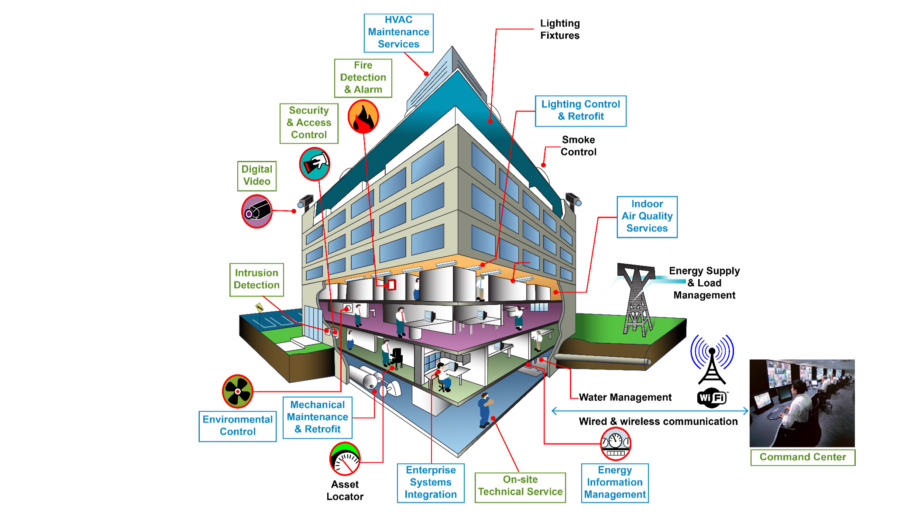
\includegraphics[width=0.9\textwidth]{figures/smart-building.jpg}
	\caption{Building Automation System schematic. Adapted from \cite{image-BAS}. }
	\label{fig:smart-building}
\end{figure}

The biggest problem in building automation is the market segmentation, where different manufactures created over the years different protocols and communication standards that didn't address solutions to all types of applications. This led to a more difficult and often impossible integration of this different approaches in the same system. Also, each vendor used to have closed specifications but, recently, in order to gain a higher margin of market, this specifications started being disclosed by vendors, which led to the appearence of new standards made from prior ones, combined. Presently the most used standards are BACnet, LonWorks, KNX and DALI. This different standards act in different \ac{bas} layers, which will be addressed in the next section. 

Though, with the rising of \ac{iot}, there have been an increasingly amount of new solutions that use high scalable technologies, well known communication standards, such as IP,  and use lightweight devices with low power consumption. This concepts will be addressed ahead in section 2.2.


\subsection{\ac{bas} Protocols}


\subsubsection{BACnet}
\subsubsection{KNX}
\subsubsection{LonWorks}
\subsubsection{DALI}
\subsubsection{EnOcean}
\subsection{\ac{bas} Solutions}
\subsubsection{Metasys \ac{bas}}
\subsubsection{Honeywell \ac{bas}}
\subsubsection{Desigo \ac{bas}}
\section{\acf{iot}}
\subsection{\acf{m2m}}
\subsection{\acf{wsan}}
\subsection{Wireless Communication Protocols}
\subsubsection{IEEE 802.15.4}
\subsubsection{6LoWPAN}
\subsubsection{ZigBee}
\subsubsection{\acf{ble}}
\subsubsection{IEEE802.11ah}
\subsubsection{Wireless Communication Protocols Comparison}
\subsection{Interaction Protocols}
\subsubsection{\acf{mqtt}}
\subsubsection{\acf{amqp}}
\subsubsection{\acf{coap}}
\subsubsection{\acf{xmpp}}
\subsubsection{Interaction Protocols Comparison}